% https://tex.stackexchange.com/a/749968/322482
\documentclass[10pt,border=0mm,tikz]{standalone}
\usetikzlibrary{calc}

\begin{document}
 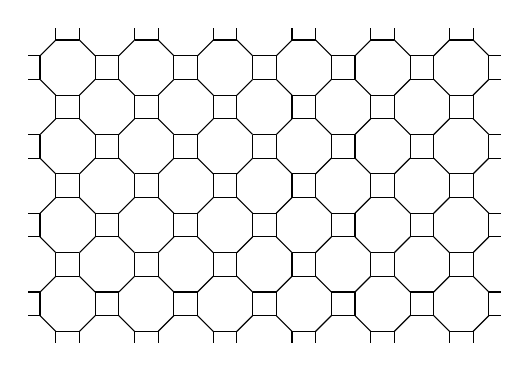
\begin{tikzpicture}[
%   line join=round,
%   line cap=round,
%   line width=1pt,
    pics/tileS/.style args={#1}{    % the small rectangle
        code={
            \def\rel{#1}
            % ~~~ reference points ~~~~~~~
            \coordinate (L) at (-.5,  0);
            \coordinate (R) at ( 0 ,-.5);
            % ~~~ invisible diagonal ~~~~~
            \draw[draw=none] (L) -- 
                    coordinate[pos=\rel]            (A)
                    coordinate[pos=\fpeval{1-\rel}] (B)
                             (R);
            % ~~~ parts of small rectangle ~~~~~~~~
            \draw (A) to (A |- L);
            \draw (A) to (A -| L);
            \draw (B) to (B |- R);
            \draw (B) to (B -| R);
            \draw (A) -- (B);
        } % end code
    }, % end pics
    % ~~~~~~~~~~~~~~~~~~~~~~~~~~~~~~~~~~~~~~~~~~~~~~~~~~~~~~~
    pics/tileA/.style args={#1}{     % composed from 4 tileS
        code={
                \foreach \a in {0,90,180,270}
                    \pic[rotate=\a] {tileS={#1}};
        } % end code
    }, % end pics
 ]
    % ~~~ let's put tiles on the floor ~~~~~~~~~~~~~~
    \foreach \x in {0,1,2,...,5}
        \foreach \y/\p in {0/.3,1/.3, % constant p-ratio
                           2/.3,3/.3} % some variation
            \pic at (\x,\y) {tileA={\p}};  
 \end{tikzpicture}
\end{document}